\documentclass[runningheads]{llncs}

% ---------------------------------------------------------------
% Include basic ECCV package
 
% TODO REVIEW: Insert your submission number below by replacing '*****'
% TODO FINAL: Comment out the following line for the camera-ready version
\usepackage[review,year=2026,ID=10551]{eccv}
% TODO FINAL: Un-comment the following line for the camera-ready version
%\usepackage{eccv}

% OPTIONAL: Un-comment the following line for a version which is easier to read
% on small portrait-orientation screens, such as mobile phones or side-by-side windows
%\usepackage[mobile]{eccv}


% ---------------------------------------------------------------
% Other packages

% Commonly used abbreviation macros are provided by eccvabbrv.
\usepackage{eccvabbrv}

% Include other packages here, before hyperref.
\usepackage{graphicx}
\usepackage{booktabs}

% The "axessiblity" package can be found at: https://ctan.org/pkg/axessibility?lang=en
\usepackage[accsupp]{axessibility}  % Improves PDF readability for those with disabilities.
 \usepackage{booktabs}
\usepackage{graphicx}
\usepackage{multirow}
\usepackage{cite}
\usepackage{color}
\usepackage{amssymb}
\usepackage{algorithm}
\usepackage{algorithmic}
\usepackage{placeins}

% ---------------------------------------------------------------
% Hyperref package

% It is strongly recommended to use hyperref, especially for the review version.
% Please disable hyperref *only* if you encounter grave issues.
% hyperref with option pagebackref eases the reviewers' job, but should be disabled for the final version.
%
% If you comment hyperref and then uncomment it, you should delete
% main.aux before re-running LaTeX.
% (Or just hit 'q' on the first LaTeX run, let it finish, and you
%  should be clear).

% TODO FINAL: Comment out the following line for the camera-ready version
%\usepackage[pagebackref,breaklinks,colorlinks,citecolor=eccvblue]{hyperref}
% TODO FINAL: Un-comment the following line for the camera-ready version
\usepackage{hyperref}

% Support for ORCID icon
\usepackage{orcidlink}


\usepackage{float}
\graphicspath{{PIC/}}
\begin{document}

% ---------------------------------------------------------------
% TODO REVIEW: Replace with your title
\title{Rectifying the Depths: A Unified Flow-Based Generative Model for Multi-Condition Underwater Enhancement} 

% TODO REVIEW: If the paper title is too long for the running head, you can set
% an abbreviated paper title here. If not, comment out.
\titlerunning{Abbreviated paper title}

% TODO FINAL: Replace with your author list. 
% Include the authors' OCRID for the camera-ready version, if at all possible.
\author{Liangfan Shi\inst{1}\orcidlink{0000-0000-0000-0000} \and
Huimin Lu\inst{2,3}\orcidlink{0000-0000-0000-0000}}

% TODO FINAL: Replace with an abbreviated list of authors.
\authorrunning{L.~Shi and H.~Lu}
% First names are abbreviated in the running head.
% If there are more than two authors, 'et al.' is used.

% TODO FINAL: Replace with your institution list.
\institute{Southeast University, Jiangsu, China\\
\email{shi.lf@seu.edu.cn} \and
Southeast University, Jiangsu, China \and
Advanced Ocean Institute of Southeast University, Nantong, Jiangsu, China\\
\email{luhuimin@ericlab.org}}

\maketitle


\begin{abstract}
Underwater imaging is severely degraded by wavelength-dependent attenuation and scattering, causing pronounced color casts, low contrast, and structural blur. We propose RF-MCUIE, a multi-condition underwater image enhancement framework based on Rectified Flow. An Adaptive Masking strategy (ADMK) dynamically localizes artifact-dominant regions for targeted restoration, improving generalization under diverse water types and degradation levels. To better align enhancement with underwater imaging physics, we incorporate background light and transmission maps as conditional guidance, constraining restoration to follow optical formation mechanisms. To overcome the high sampling cost of diffusion-style models, we learn a rectified transport path with an approximately straight probability trajectory from noise to the data manifold, enabling high-fidelity enhancement in only three inference steps. Extensive evaluations on LSUI, UIEB, and U45 demonstrate state-of-the-art performance, effectively neutralizing color deviations and recovering fine details with high computational efficiency.
\keywords{Underwater image enhancement \and Rectified Flow \and Diffusion models \and Physical priors}
\end{abstract}

% !TeX root = ../main.tex
\section{Introduction}
\label{sec:intro}

Underwater optical imaging is inevitably degraded by wavelength-dependent absorption and scattering, which jointly cause contrast attenuation, haze-like veiling light, detail blur, and severe color casts \cite{r1,r12}. Such degradations not only deteriorate human perception but also directly undermine the reliability of underwater machine vision for autonomous inspection, navigation, and manipulation \cite{r2,r3}. Therefore, underwater image enhancement (UIE) remains a fundamental yet challenging prerequisite for robust underwater robotic perception.

Over the past decade, UIE has evolved from hand-crafted priors and physics-inspired inversion \cite{r4,r14,r17} to learning-based enhancement driven by curated benchmarks and increasingly powerful backbones \cite{r18,r6}. Modern deep models, including attention-enhanced CNNs and Transformers, improve global color consistency and local detail recovery \cite{r0,r42,r7}. Nevertheless, the practical deployment of UIE models still faces persistent difficulties. Training supervision is often imperfect because of the synthetic-to-real gap, noisy ``reference'' images, and local over-enhancement artifacts, which can mislead optimization and harm generalization. Purely data-driven mappings may also underutilize physical cues such as background light and depth-dependent attenuation, leading to unstable color correction in diverse water types and lighting conditions.

Recently, diffusion-based generative models have become a frontier paradigm for low-level vision because of their strong learned priors and texture synthesis capability \cite{r20,r22}. Several works have started to adapt conditional diffusion to underwater enhancement and demonstrate impressive perceptual quality \cite{r9,r24,r8,r10}. However, standard diffusion sampling typically requires dozens to hundreds of iterative denoising steps, which results in considerable latency and energy consumption; even with accelerated solvers or distillation, efficient deployment on embedded underwater platforms remains non-trivial \cite{r21,r43,r45,r46}.

To address these challenges, we propose \emph{RF-MCUIE}, a \textbf{M}ulti-\textbf{C}ondition \textbf{U}nderwater \textbf{I}mage \textbf{E}nhancement framework based on \textbf{R}ectified \textbf{F}low \cite{r11}. Compared with diffusion models, rectified flow learns a nearly straight transport dynamics that enables high-quality generation with remarkably few function evaluations, offering a favorable quality--efficiency trade-off \cite{r30,r49}. In addition, we inject physics-guided conditions into the generative process to better conform to underwater image formation through distance-independent background light estimation DBLE, and we introduce an adaptive masking strategy to reduce the negative impact of unreliable training regions. Fig.~\ref{fig:intro_tradeoff} summarizes the resulting quality--efficiency characteristics.

\begin{figure}[t]
    \centering
    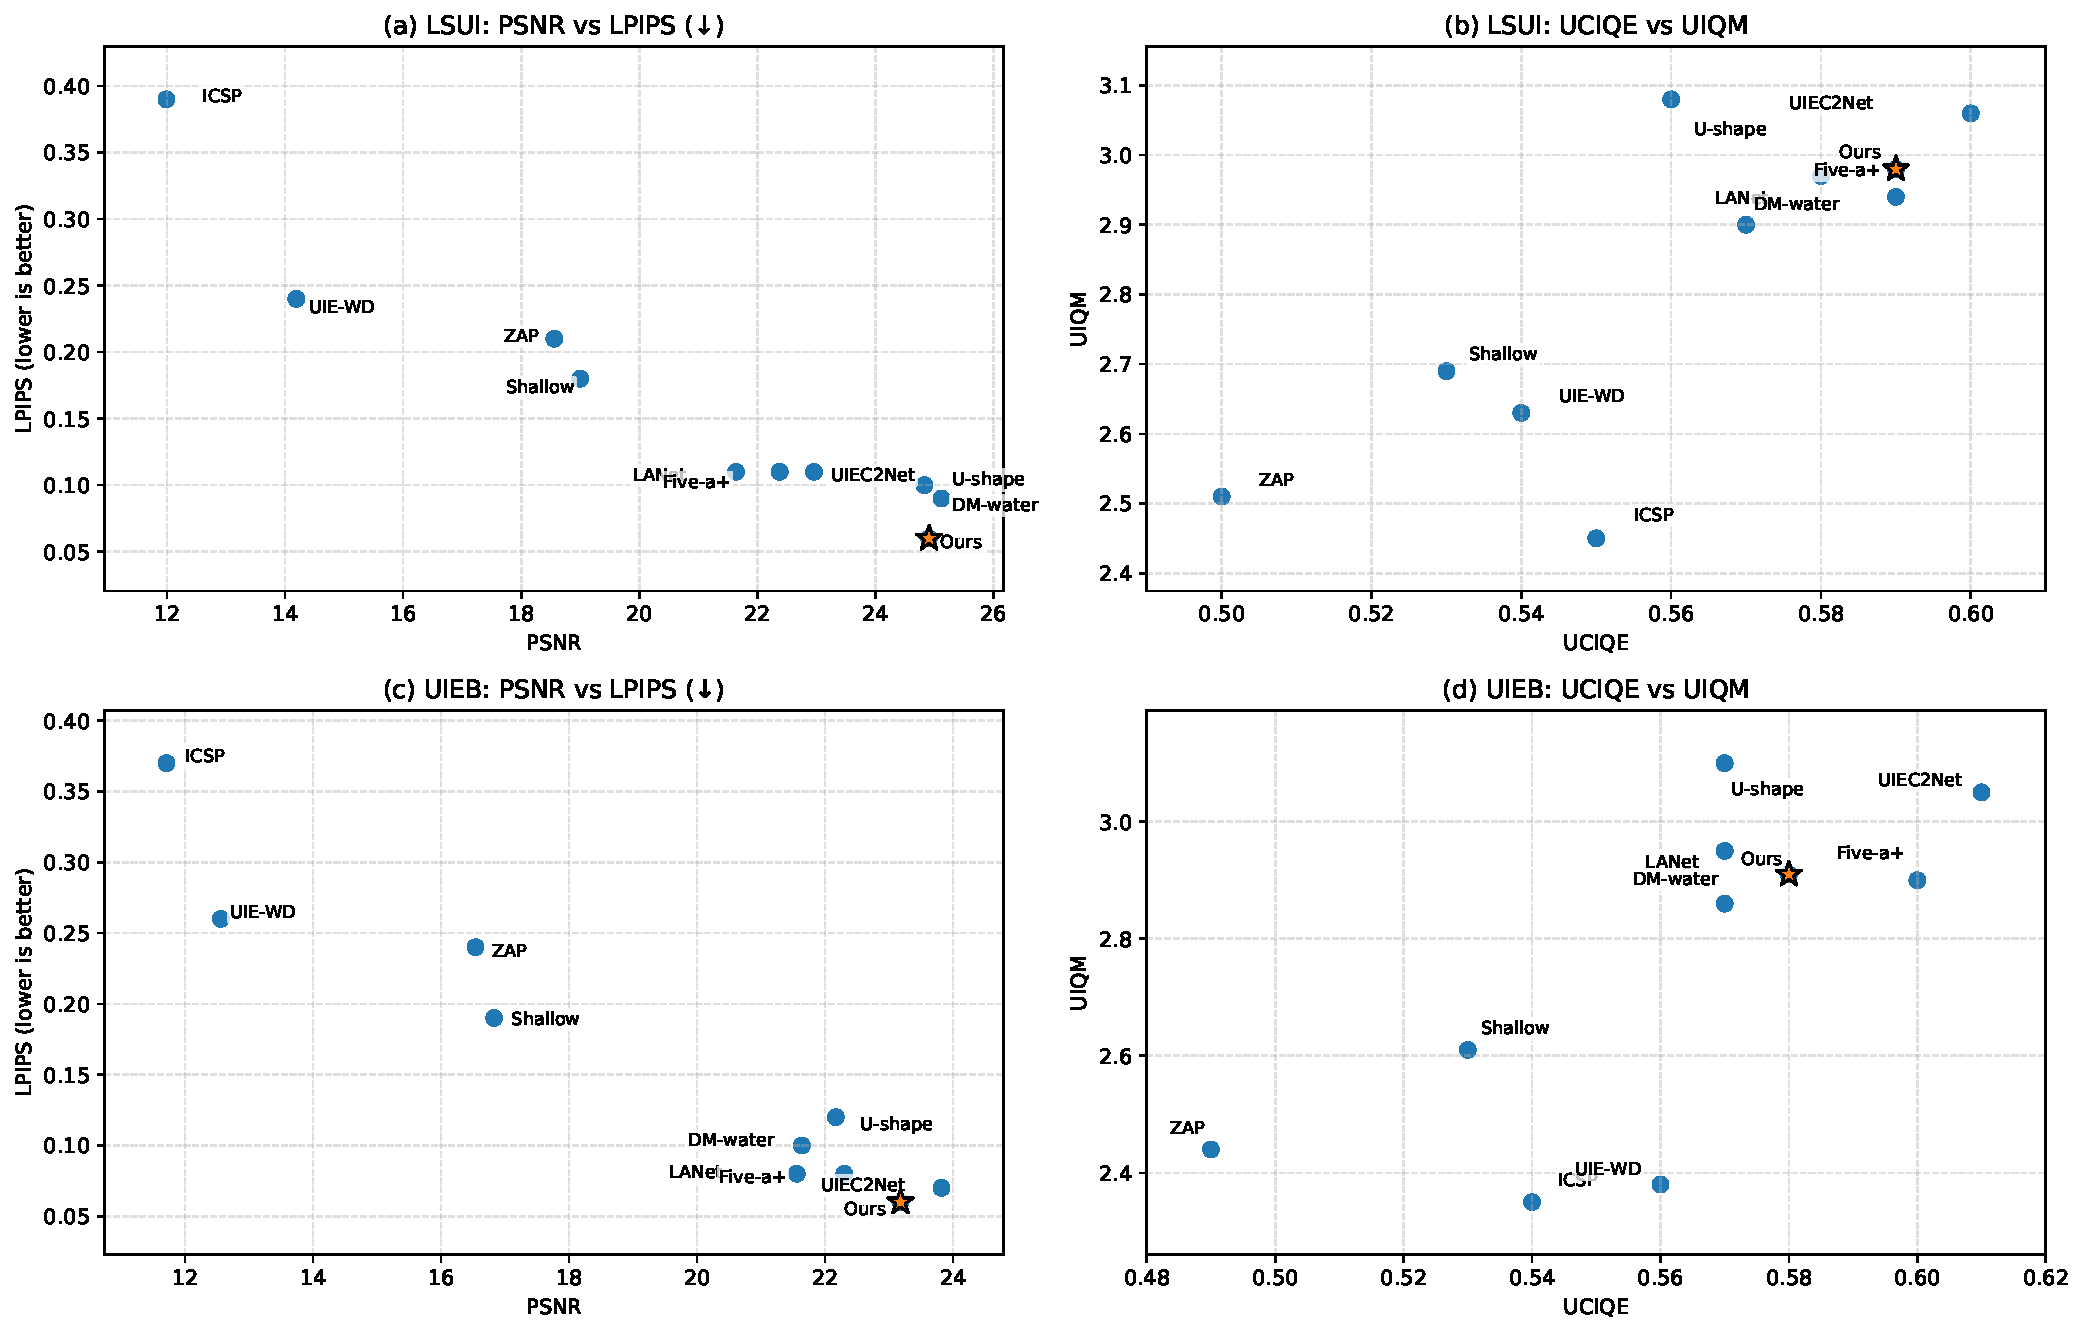
\includegraphics[width=\linewidth]{fig_tradeoff_scatter.pdf}
    \caption{Restoration quality--efficiency trade-off of representative methods. RF-MCUIE achieves a favorable balance with low perceptual error and low computational cost.}
    \label{fig:intro_tradeoff}
\end{figure}

Despite rapid progress, UIE still suffers from limited real paired data, strong domain shifts across water types and devices, and evaluation protocols that are weakly aligned with downstream tasks such as detection and SLAM \cite{r6,r18}. Designing physically consistent, efficient, and task-aware enhancement models remains an open direction for future research.

The main contributions are summarized as follows:
\begin{itemize}
    \item \textbf{Adaptive masking for reliable supervision.} We propose an Adaptive Masking (ADMK) strategy that detects sub-optimally enhanced local regions via multi-color-space discrepancies and suppresses their influence during training, improving stability and generalization.
    \item \textbf{Physics-guided multi-condition rectified flow.} We introduce distance-independent background light estimation DBLE and build an efficient rectified-flow-based enhancement network conditioned on physically meaningful cues, including background light and transmission-related maps, enabling robust dehazing and color correction across diverse underwater conditions.
    \item \textbf{Quality--efficiency oriented optimization.} A composite objective combining flow regression, structural similarity, and perceptual constraints is adopted to enhance fine textures while maintaining faithful structure under few-step inference.
\end{itemize}


% !TeX root = ../main.tex
\section{Related Work}

\subsection{Underwater Image Enhancement}
Early UIE research predominantly relied on physics-inspired modeling and hand-crafted priors. Based on the Jaffe--McGlamery image formation model, many methods estimate background light and medium transmission to invert attenuation and backscatter effects \cite{r12,r4,r14}, while non-physical approaches improve perceptual quality by manipulating intensity and color statistics such as histogram equalization and Retinex-style illumination correction \cite{r15,r17}. With public benchmarks and improved training recipes, deep learning has become the dominant paradigm \cite{r18,r6}, and representative CNN and Transformer designs improve detail recovery, global color consistency, and contrast \cite{r0,r7}. Hybrid methods further inject medium-dependent cues such as transmission or multi-color embeddings to enhance robustness \cite{r42,r40,r41}, but UIE models still suffer from local over-enhancement, unstable color correction, and performance degradation under unseen conditions.

\subsection{Diffusion Models}
Diffusion models have achieved strong performance in image synthesis and restoration by iterative denoising with powerful learned priors \cite{r20,r52,r21}, and their flexibility has enabled diverse conditional generation frameworks for low-level vision \cite{r22}. In underwater enhancement, recent studies use conditional diffusion to improve texture realism and color restoration, sometimes with physical priors or Transformer backbones for better robustness \cite{r9,r24,r8,r10}. The main limitation is efficiency, because conventional diffusion requires many sequential sampling steps. Existing acceleration strategies include improved solvers \cite{r43,r44}, latent diffusion \cite{r47}, and distillation or consistency training for one- or few-step inference \cite{r45,r46,r48}, yet deployment on resource-constrained underwater platforms remains difficult due to model size, iterative computation, and unstable conditioning across diverse water environments.

\subsection{Rectified Flow}
Rectified flow provides an efficient alternative by learning deterministic transport from noise to data through a regression-style objective, enabling fast ODE sampling with fewer function evaluations than diffusion \cite{r11}. Related formulations such as stochastic interpolants and flow matching further improve stability and controllability \cite{r28,r29}, and recent results in InstaFlow and FlowIE show that one-step or few-step generation can retain strong perceptual quality in practical enhancement pipelines \cite{r30,r49}. Although low-step performance continues to improve through better training and parameterization strategies \cite{r50,r51}, underwater enhancement is still challenging because of limited real paired supervision, large water-type variation, and unreliable physical cue estimation; these factors can amplify artifacts when efficient generative models are conditioned incorrectly. This motivates our design that combines rectified flow with physics-guided multi-condition inputs and adaptive masking for more stable restoration.


% !TeX root = ../main.tex
\section{Method}
\label{sec:method}

\subsection{Overall Architecture}
\label{subsec:overall_architecture}

RF-MCUIE is designed for underwater scenes with mixed degradations, including wavelength-dependent attenuation, spatially varying scattering, and color bias under different water types. The framework combines physical-condition construction and conditional rectified flow transport in a unified pipeline. As shown in \cref{fig:overall_arch}, the full system consists of an adaptive preprocessing module and a multi-condition rectified flow enhancement network.

\begin{figure}[tb]
    \centering
    \makebox[\linewidth][c]{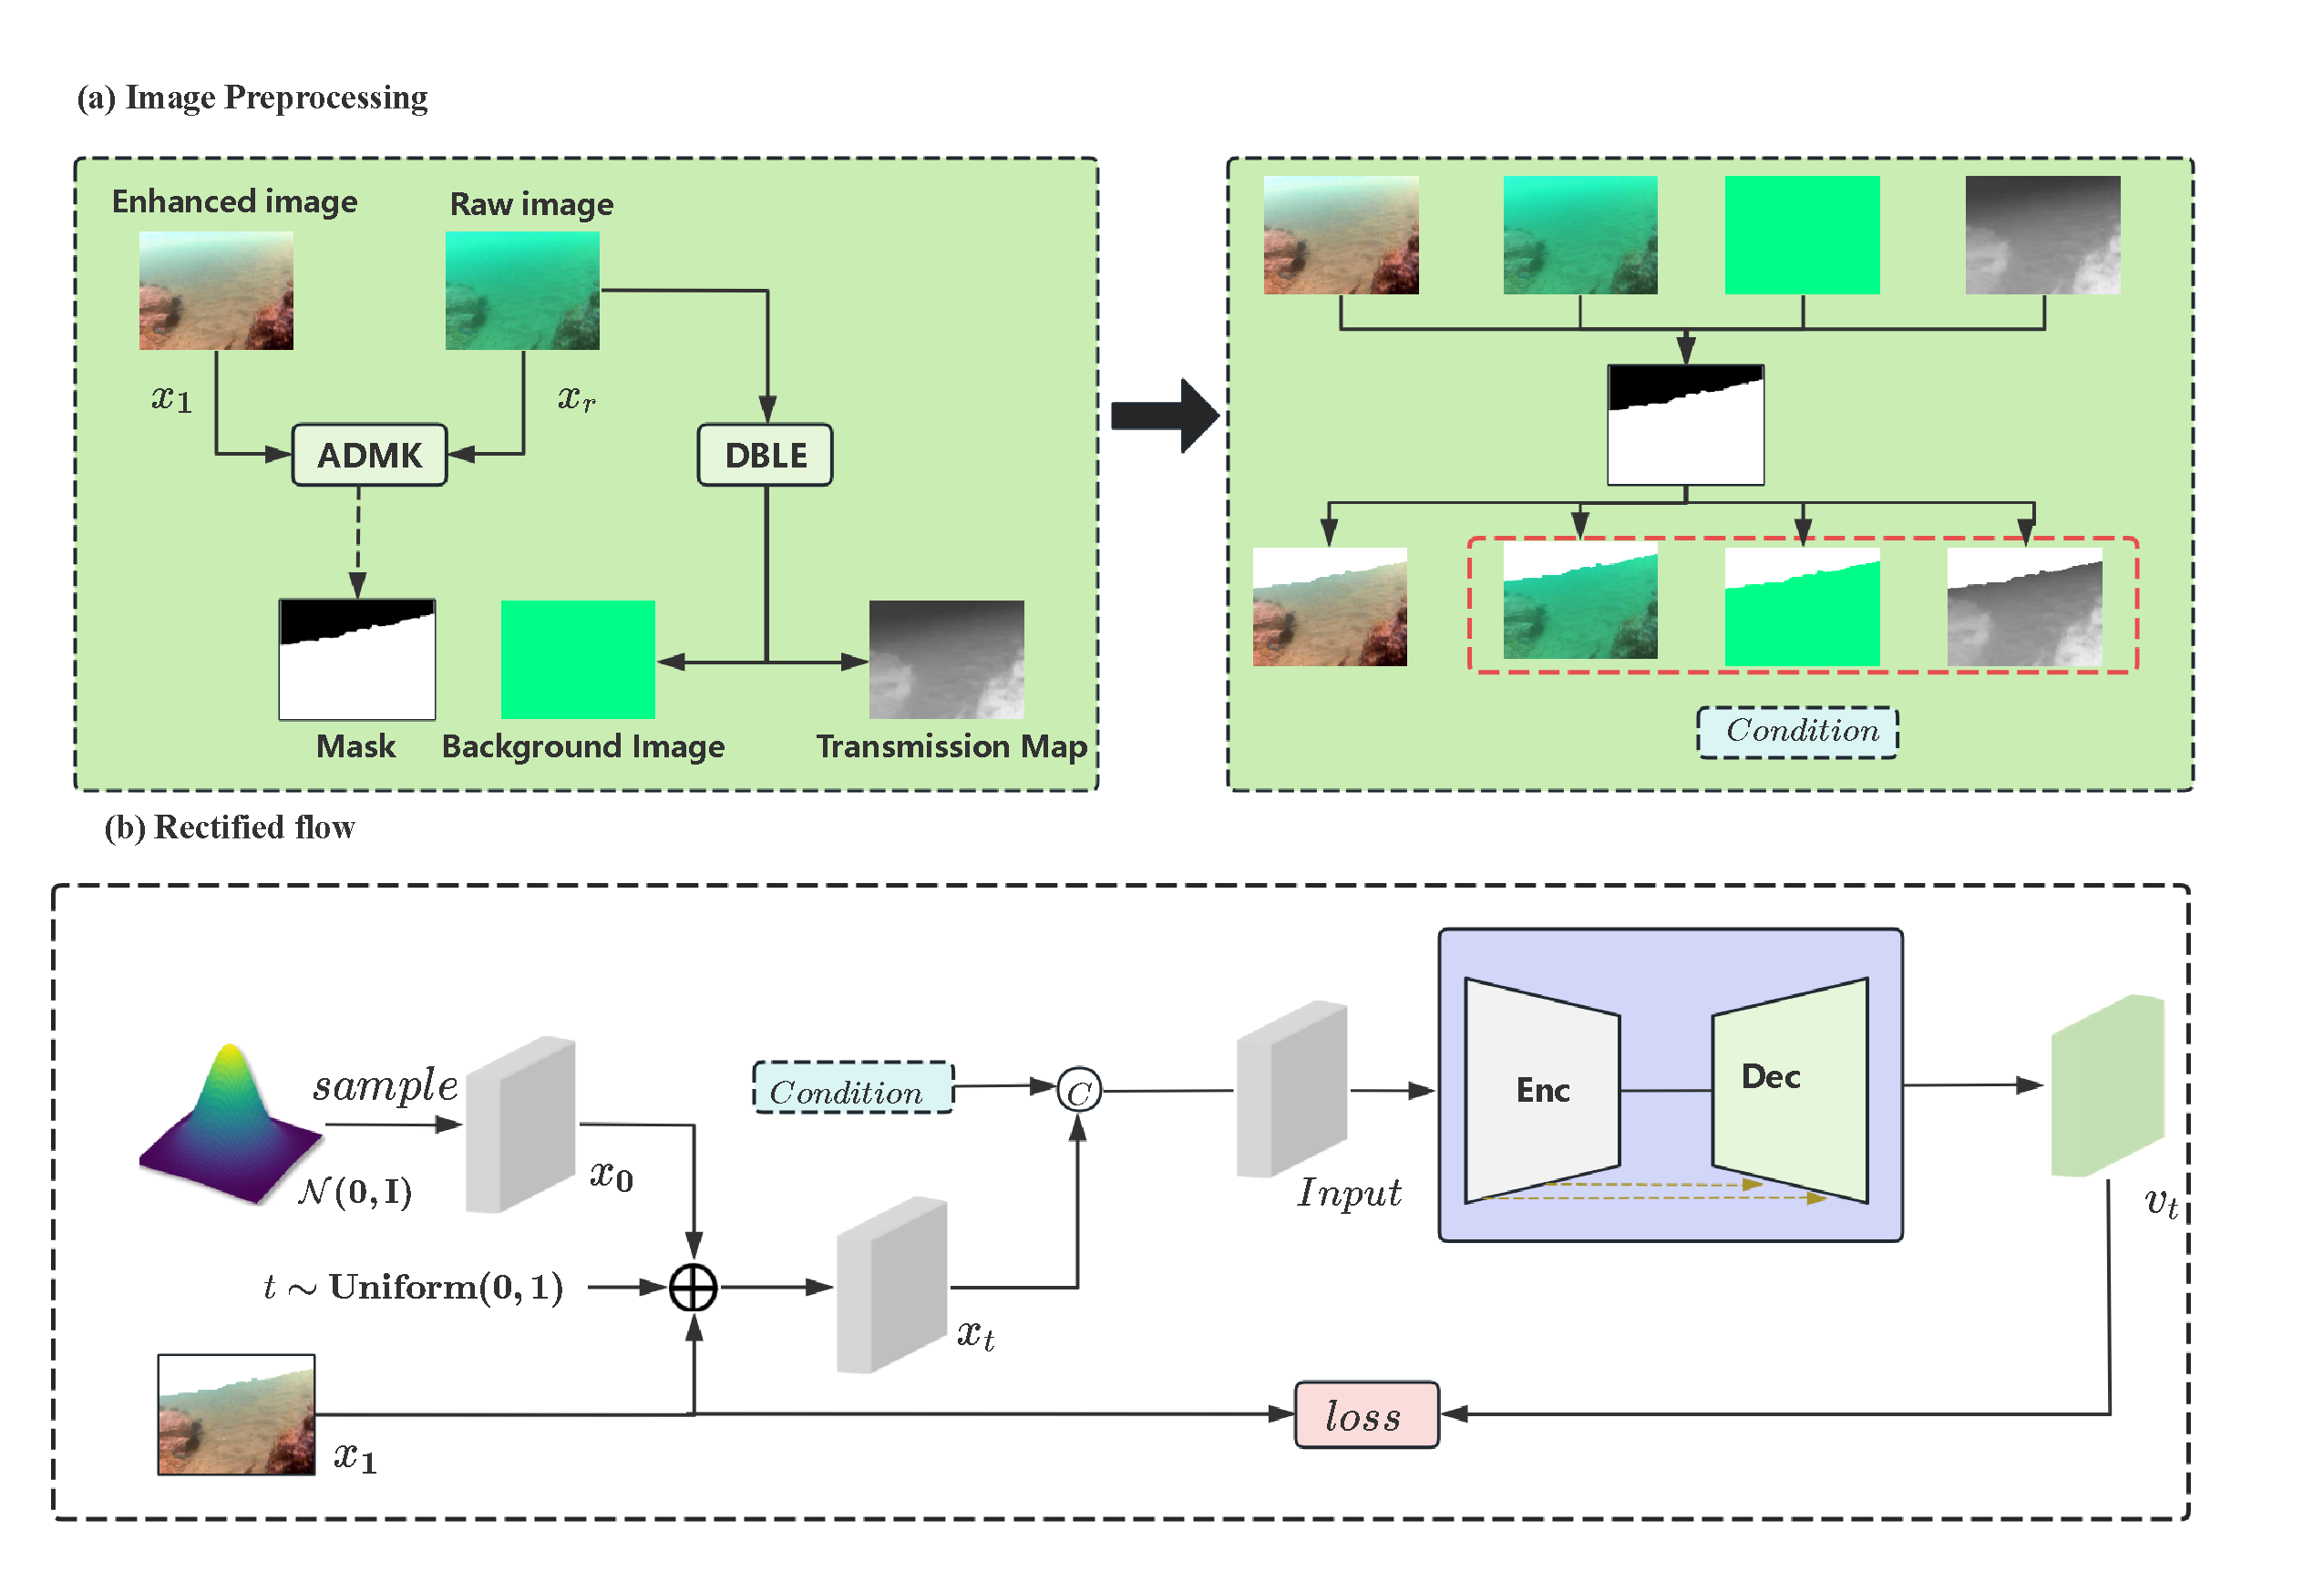
\includegraphics[width=1.06\linewidth]{fig1.pdf}}
    \caption{Overall framework of RF-MCUIE, including adaptive preprocessing and multi-condition rectified flow enhancement.}
    \label{fig:overall_arch}
\end{figure}

During preprocessing, the model estimates physically meaningful priors from the raw input and filters unreliable supervision areas. These outputs are fused into a condition tensor that is injected into the flow network at training and inference time. During generation, the network learns a direct transport from noise to the enhanced image manifold under these conditions, which reduces iterative denoising overhead while preserving fine structures and color consistency.

\subsubsection{Problem Formulation and Multi-Condition Inputs}
Given a raw underwater image $I_{raw}\in[0,1]^{H\times W\times 3}$, the objective is to recover a visually clear image $J$ with improved structure and color fidelity. The imaging process is modeled as
\begin{equation}
I_{raw}^{c}(\mathbf{x}) = J^{c}(\mathbf{x})\,T^{c}(\mathbf{x}) + B^{c}(\mathbf{x})\bigl(1-T^{c}(\mathbf{x})\bigr),
\label{eq:uw_imaging_model}
\end{equation}
where $B$ and $T$ denote the background-light component and transmission component. In practice, direct inversion is unstable in diverse marine environments, especially when depth, turbidity, and illumination vary simultaneously. RF-MCUIE therefore uses estimated physical maps as soft constraints instead of relying on explicit inverse reconstruction.

Specifically, the DBLE module estimates background light and transmission from $I_{raw}$, and ADMK provides a binary reliability mask $\mathcal{M}$ for robust supervision. The condition tensor is built by masked concatenation:
\begin{equation}
C = \mathrm{Concat}\!\bigl(\mathcal{M}\odot I_{raw},\ \mathcal{M}\odot B,\ \mathcal{M}\odot T\bigr),
\label{eq:cond_concat_overview}
\end{equation}
which jointly encodes appearance information and physics-related priors. This condition design encourages the network to focus on valid regions and suppresses the influence of low-quality pseudo targets.

\subsubsection{Conditional Rectified Flow Formulation}
Conditioned on $C$, RF-MCUIE learns a transport path from Gaussian noise to the clear-image manifold. The generation dynamics are defined by
\begin{equation}
\frac{dX_t}{dt} = v_{\theta}(X_t, C, t),\qquad X_0\sim\mathcal{N}(0,\mathbf{I}),\ t\in[0,1],
\label{eq:rf_ode}
\end{equation}
where $v_{\theta}$ is parameterized by a U-Net backbone. The final state $X_1$ is treated as the enhanced result. Compared with diffusion-style sampling that requires many reverse steps, the rectified flow trajectory is directly optimized for efficient transport, so high-quality restoration can be obtained with only a few integration steps.

\subsection{Adaptive Masking (ADMK) Strategy}
Public underwater datasets usually provide reference images produced by traditional or early deep models. These references improve supervision availability but may include local artifacts, over-enhancement, or chromatic drift. If all pixels are treated equally during optimization, the model can overfit these errors and amplify unstable regions. ADMK addresses this issue by constructing a reliability-aware training mask.

\begin{figure}[H]
    \centering
    \vspace{-0.4cm}
    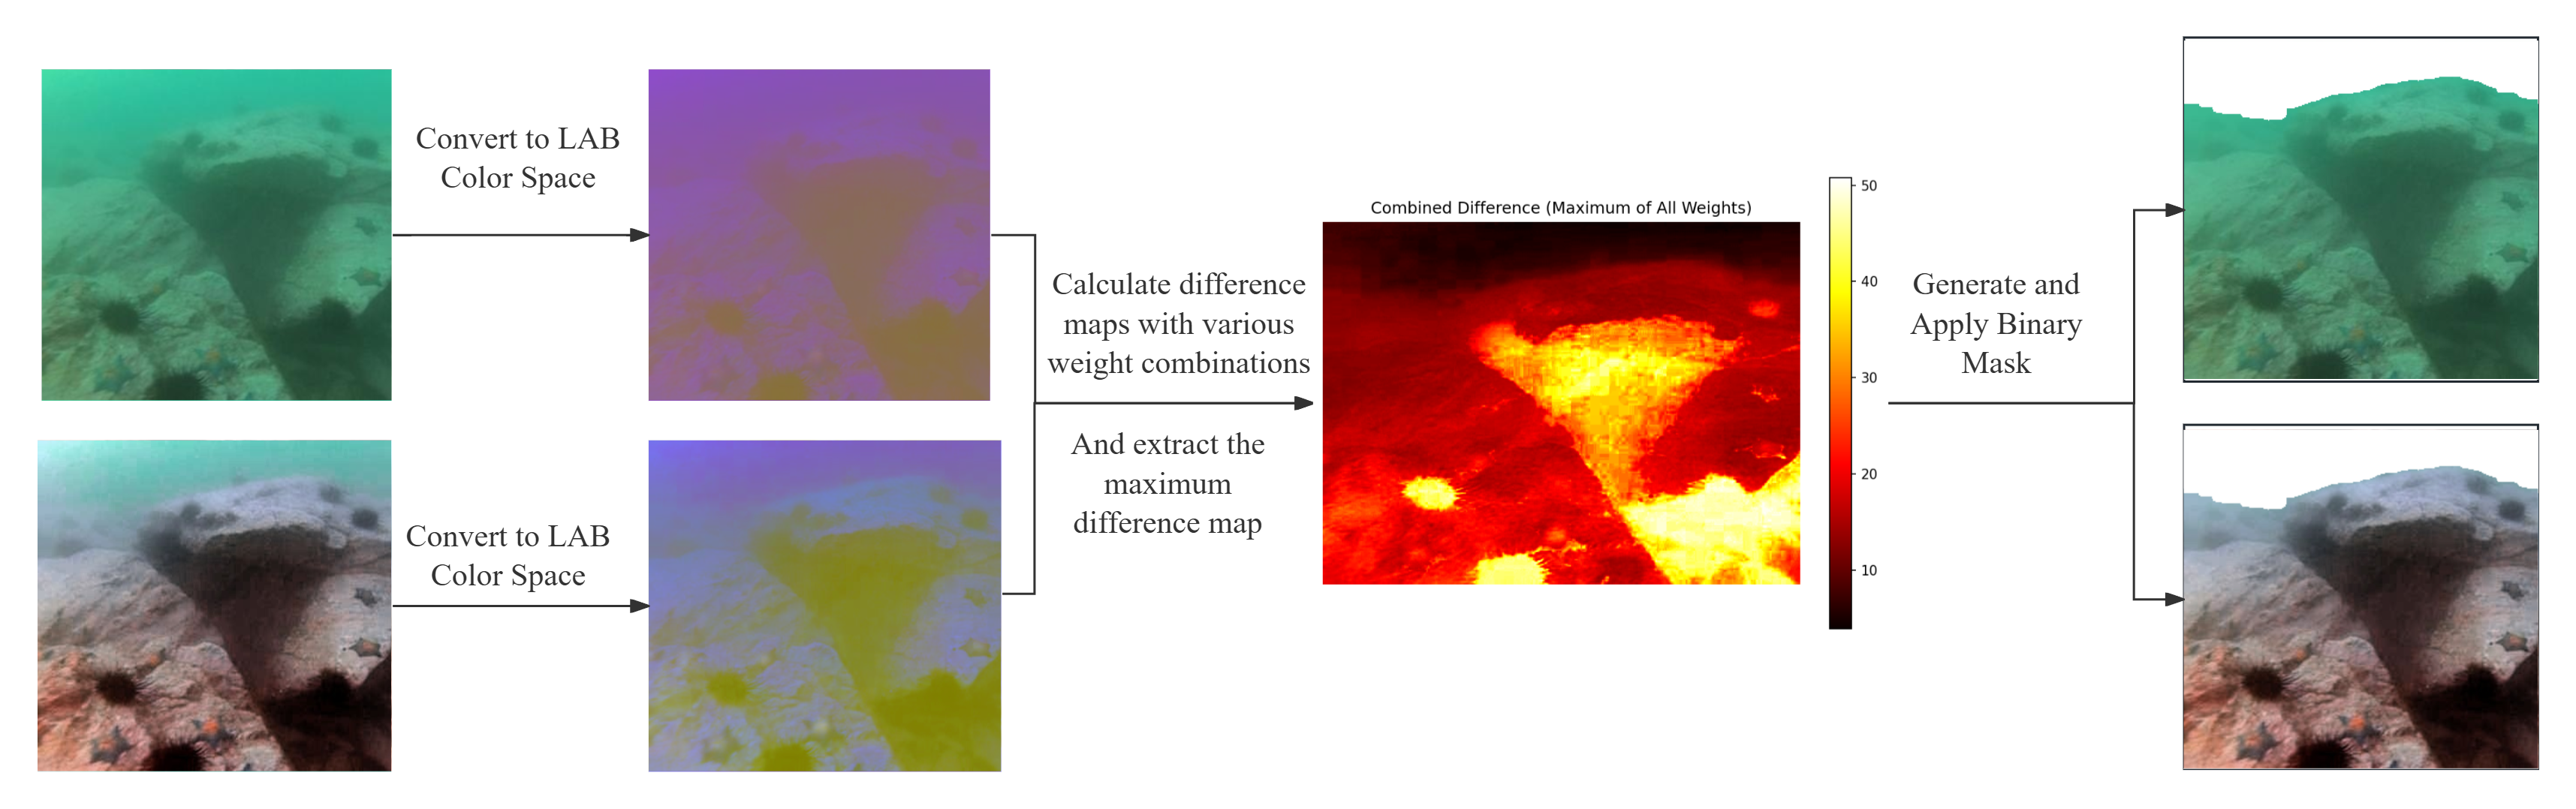
\includegraphics[width=\linewidth]{fig2.png}
    \caption{Generation pipeline of Adaptive Masking (ADMK).}
    \label{fig:admk}
    \vspace{-0.4cm}
\end{figure}

ADMK first converts $I_{raw}$ and the reference image $I_{enh}$ to LAB space and computes channel-wise discrepancy maps. A multi-weight projection then aggregates these differences:
\begin{equation}
\Delta_{gray}(\mathbf{x}) = \max_{k\in\{1,\dots,K\}}\left(\omega_L^k\Delta L(\mathbf{x}) + \omega_A^k\Delta A(\mathbf{x}) + \omega_B^k\Delta B(\mathbf{x})\right).
\label{eq:admk_gray}
\end{equation}
This max-projection mechanism improves robustness to different artifact patterns because luminance and chromatic deviations are emphasized with different weights.

After Gaussian smoothing, ADMK applies thresholding to obtain the binary mask:
\begin{equation}
\mathcal{M}(\mathbf{x}) =
\begin{cases}
1, & \text{if } (G_{\sigma} * \Delta_{gray})(\mathbf{x}) > \tau,\\
0, & \text{otherwise}.
\end{cases}
\label{eq:admk_binary}
\end{equation}
Pixels with value 1 are treated as reliable supervision regions in both condition construction and loss computation. Adaptive threshold statistics and morphological post-processing are reported in Supplementary A.

\subsection{Distance-independent Background Light Estimation (DBLE)}
\label{subsec:dble}

DBLE extracts physically interpretable priors without explicit metric depth estimation. The design follows two principles: the background-light field varies slowly in space, while transmission is tied to local visibility attenuation. Based on these principles, DBLE computes a smooth background map and a refined transmission map that are later injected into the condition tensor.

The background-light component is estimated with guided filtering:
\begin{equation}
B^c = \mathrm{GF}(I_{raw}^c; g, r_B, \epsilon_B),\qquad c\in\{r,g,b\},
\label{eq:dble_B_main}
\end{equation}
where $g$ is the guidance image, $r_B$ is the filter radius, and $\epsilon_B$ controls edge preservation strength. This operation keeps large-scale illumination trends while suppressing texture-level noise.

Using the estimated $B$, DBLE computes a coarse transmission by normalized local dark response:
\begin{equation}
T_0(\mathbf{x}) = 1 - \omega\!\left(\min_{\mathbf{y}\in\Omega(\mathbf{x})}\ \min_{c\in\{r,g,b\}}\frac{I_{raw}^{c}(\mathbf{y})}{B^{c}(\mathbf{y})+\epsilon}\right),
\label{eq:dble_T0_main}
\end{equation}
where $\omega$ controls attenuation strength and $\Omega(\mathbf{x})$ is a local window. The resulting map is further refined by guided filtering to preserve object boundaries and suppress halo artifacts. Full derivations, including channel-wise transmission extension and coarse restoration expressions, are provided in Supplementary A.

\subsection{Multi-Condition Rectified Flow Network}
With condition tensor $C$, the network is trained by pairing source noise and target reference images. We sample $X_0\sim\mathcal{N}(0,\mathbf{I})$ and define the interpolation state
\begin{equation}
X_t = tX_1 + (1-t)X_0,\qquad t\sim\mathcal{U}(0,1),
\label{eq:rf_xt}
\end{equation}
then regress the straight transport velocity:
\begin{equation}
\min_{\theta}\ \mathbb{E}_{X_0,X_1,t}\left[\left\|v_{\theta}(X_t,C,t) - (X_1-X_0)\right\|^2\right].
\label{eq:rf_mse}
\end{equation}
This objective encourages the network to learn a stable global direction from degraded observations to enhanced outputs under physical conditions.

During inference, we discretize \cref{eq:rf_ode} with Euler integration:
\begin{equation}
X_{t_{i+1}} = X_{t_i} + v_{\theta}(X_{t_i}, C, t_i)\,\Delta t,\qquad \Delta t=\frac{1}{n}.
\label{eq:euler}
\end{equation}
Small $n$ gives fast inference, while moderate multi-step integration improves local detail restoration.

\begin{figure}[H]
    \centering
    \vspace{-0.4cm}
    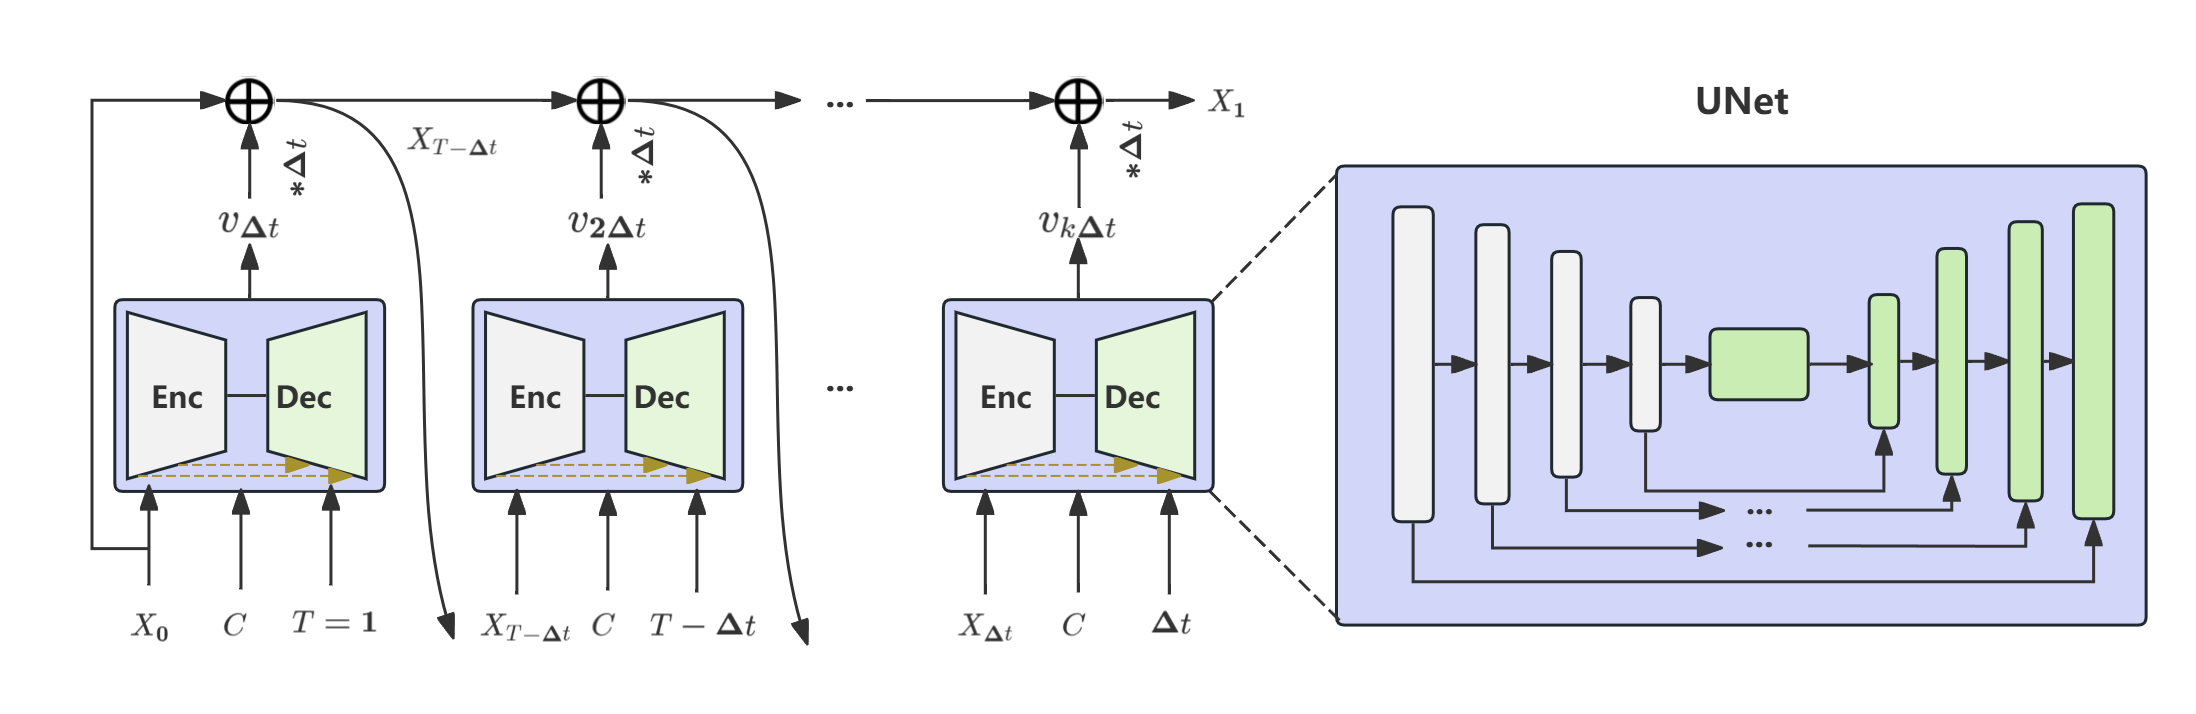
\includegraphics[width=\linewidth]{fig3.png}
    \caption{Denoising and transport process in the multi-condition rectified flow network.}
    \label{fig:flow_process}
    \vspace{-0.4cm}
\end{figure}

\subsection{Composite Loss Function and Two-Stage Training Strategy}
The training objective combines transport learning and image-domain quality constraints. The core term is the mask-aware velocity regression loss:
\begin{equation}
\mathcal{L}_{flow} = \mathbb{E}_{X_0,X_1,t}\left[\frac{\left\|\mathcal{M}\odot\bigl(v_{\theta}(X_t,C,t)-(X_1-X_0)\bigr)\right\|_2^2}{\|\mathcal{M}\|_1+\varepsilon}\right].
\label{eq:lflow_masked}
\end{equation}
On top of this term, structural similarity, perceptual consistency, and LAB color-consistency losses are added to improve texture sharpness and chromatic stability.

The total objective is
\begin{equation}
\mathcal{L}_{total} = \mathcal{L}_{flow} + \lambda_1\mathcal{L}_{SSIM} + \lambda_2\mathcal{L}_{per} + \lambda_3\mathcal{L}_{color}.
\label{eq:ltotal}
\end{equation}
Optimization is performed in two stages. The first stage focuses on $\mathcal{L}_{flow}$ to stabilize transport geometry, and the second stage enables the full objective to refine visual quality. The transition schedule for reconstruction weights is
\begin{equation}
\lambda_i(e) = \frac{\lambda_i^{max}}{1 + \exp\left(-\frac{e - e_0}{\kappa}\right)},\qquad i\in\{1,2,3\}.
\label{eq:lambda_schedule}
\end{equation}
Detailed reconstruction formulas and additional implementation settings are reported in Supplementary A and Supplementary C.


% !TeX root = ../main.tex
\section{Experiments and Results}
\label{sec:experiments}
\subsection{Experimental Settings}
\newcommand{\best}[1]{\textcolor{red}{#1}}
\newcommand{\second}[1]{\textcolor{blue}{#1}}

To comprehensively evaluate the proposed RF-MCUIE network, experiments are conducted on three public underwater datasets: LSUI~\cite{r7}, UIEB~\cite{r18}, and U45~\cite{r53}.  For LSUI and UIEB, evaluation metrics include PSNR, SSIM~\cite{r31}, LPIPS~\cite{r34}, FID~\cite{r35}, UCIQE~\cite{r36}, and UIQM~\cite{r37}, while only UIQM and UCIQE are employed for U45. The model is implemented in PyTorch 1.8 \cite{r38} and trained on a single NVIDIA RTX A6000 GPU. Input images are cropped to $256 \times 256$ and normalized to $[-1, 1]$. We adopt the Adam optimizer \cite{r39} ($\beta_1=0.9$, $\beta_2=0.999$) with a learning rate of $1 \times 10^{-4}$ and a batch size of 8, training the network for $1,000,000$ iterations. To balance efficiency and stability, the Rectified Flow inference step $n$ is set to 1 during training and 3 during testing. Furthermore, a two-stage training strategy is adopted: an initial coarse recovery using a pixel-level MSE loss, followed by fine-tuning with perceptual and structural losses.

\subsection{Comparison with State-of-the-Art Methods}

We comprehensively evaluate the proposed RF-MCUIE network against representative underwater image enhancement baselines, including optimization-based methods ZAP~\cite{r57}, ICSP~\cite{r56}, and Shallow~\cite{r58}, as well as learning-based approaches UIE-WD~\cite{r54}, DM-water~\cite{r24}, LANet~\cite{r55}, UIEC2Net~\cite{r41}, FiveA$^{+}$Net~\cite{r59}, and U-shape transformer~\cite{r7}.  For qualitative analysis, six typical degraded images are shown in Figure \ref{fig:qualitative_comp}. The first three rows exhibit greenish casts with compressed contrast, while the bottom three are bluish with heavy scattering. Traditional methods such as ZAP and ICSP often under-correct greenish scenes and fail to balance dehazing with color regression in bluish ones. Deep learning methods like UIE-WD can cause over-saturation, and DM-water or LANet still exhibit noticeable green residue and color drift. In contrast, our model effectively neutralizes color shifts, restores texture details, and significantly improves visibility under heavy scattering, demonstrating comprehensive advantages in color correction and structural consistency.
% 表1：LSUI 数据集对比
\begin{table}[htbp]
    \centering
    \small 
    \caption{Quantitative comparison on LSUI. Red indicates the best value, blue indicates the second best value, and bold highlights our method only.}
    \label{tab:lsui}
    \begin{tabular*}{\linewidth}{@{\extracolsep{\fill}}lcccccc}
        \toprule
        Method & UCIQE $\uparrow$ & UIQM $\uparrow$ & PSNR $\uparrow$ & SSIM $\uparrow$ & LPIPS $\downarrow$ & FID $\downarrow$ \\
        \midrule
        ICSP~\cite{r56} & 0.55 & 2.45 & 11.99 & 0.55 & 0.39 & 92.12 \\
        ZAP~\cite{r57} & 0.50 & 2.51 & 18.56 & 0.79 & 0.21 & 62.35 \\
        UIEC2Net~\cite{r41} & \best{0.60} & \second{3.06} & 22.96 & 0.86 & 0.11 & 40.42 \\
        LANet~\cite{r55} & 0.58 & 2.97 & 21.64 & 0.86 & 0.11 & 37.58 \\
        Shallow~\cite{r58} & 0.53 & 2.69 & 19.00 & 0.79 & 0.18 & 48.37 \\
        UIE-WD~\cite{r54} & 0.54 & 2.63 & 14.19 & 0.69 & 0.24 & 79.55 \\
        FiveA$^{+}$Net~\cite{r59} & \second{0.59} & 2.94 & 22.38 & 0.86 & 0.11 & 37.78 \\
        U-shape~\cite{r7} & 0.56 & \best{3.08} & 24.83 & 0.87 & 0.10 & \second{31.49} \\
        DM-water~\cite{r24} & 0.57 & 2.90 & \best{25.12} & \second{0.88} & \second{0.09} & 32.54 \\
        \midrule
        \textbf{Ours} & \textbf{\second{0.59}} & \textbf{2.98} & \textbf{\second{24.91}} & \textbf{\best{0.90}} & \textbf{\best{0.06}} & \textbf{\best{26.69}} \\
        \bottomrule
    \end{tabular*}
\end{table}

We conduct comprehensive quantitative evaluations on the LSUI and UIEB test sets, summarized in Tables \ref{tab:lsui} and \ref{tab:uieb}. While some deep learning methods perform decently on PSNR, our method achieves the most competitive overall performance, notably securing the lowest scores in the perceptual metrics with LPIPS of 0.06 and FID of 26.69 on the LSUI dataset. This proves that integrating Rectified Flow with physical priors generates results with higher visual quality. On the UIEB dataset, our method similarly maintains optimal perceptual performance and leads in no-reference metrics UCIQE and UIQM, verifying its superiority in restoring details.


% 表2：UIEB 数据集对比
\begin{table}[htbp]
    \centering
    \small 
    \caption{Quantitative comparison on UIEB. Red indicates the best value, blue indicates the second best value, and bold highlights our method only.}
    \label{tab:uieb}
    \begin{tabular*}{\linewidth}{@{\extracolsep{\fill}}lcccccc}
        \toprule
        Method & UCIQE $\uparrow$ & UIQM $\uparrow$ & PSNR $\uparrow$ & SSIM $\uparrow$ & LPIPS $\downarrow$ & FID $\downarrow$ \\
        \midrule
        ICSP~\cite{r56} & 0.54 & 2.35 & 11.71 & 0.53 & 0.37 & 122.35 \\
        ZAP~\cite{r57} & 0.49 & 2.44 & 16.54 & 0.74 & 0.24 & 62.65 \\
        UIEC2Net~\cite{r41} & \best{0.61} & \second{3.05} & \best{23.82} & \best{0.87} & \second{0.07} & 30.01 \\
        LANet~\cite{r55} & 0.57 & 2.95 & 21.56 & \second{0.85} & 0.08 & \second{29.95} \\
        Shallow~\cite{r58} & 0.53 & 2.61 & 16.83 & 0.72 & 0.19 & 59.68 \\
        UIE-WD~\cite{r54} & 0.56 & 2.38 & 12.56 & 0.62 & 0.26 & 104.32 \\
        FiveA$^{+}$Net~\cite{r59} & \second{0.60} & 2.90 & 22.30 & 0.86 & 0.08 & 36.60 \\
        U-shape~\cite{r7} & 0.57 & \best{3.10} & 22.17 & 0.82 & 0.12 & 38.91 \\
        DM-water~\cite{r24} & 0.57 & 2.86 & 21.64 & 0.82 & 0.10 & 33.08 \\
        \midrule
        \textbf{Ours} & \textbf{0.58} & \textbf{2.91} & \textbf{\second{23.18}} & \textbf{\best{0.87}} & \textbf{\best{0.06}} & \textbf{\best{28.78}} \\
        \bottomrule
    \end{tabular*}
\end{table}
% 表3：U45 数据集对比
\begin{table}[htbp]
    \centering
    \small 
    \caption{Quantitative comparison on U45. Red indicates the best value, blue indicates the second best value, and bold highlights our method only.}
    \label{tab:u45}
    \begin{tabular*}{\linewidth}{@{\extracolsep{\fill}}lcc}
        \toprule
        Method & UCIQE $\uparrow$ & UIQM $\uparrow$ \\
        \midrule
        ICSP~\cite{r56} & 0.53 & 1.98 \\
        ZAP~\cite{r57} & 0.49 & 2.79 \\
        UIEC2Net~\cite{r41} & \second{0.61} & \best{3.40} \\
        LANet~\cite{r55} & \best{0.63} & 3.29 \\
        Shallow~\cite{r58} & 0.53 & 2.80 \\
        UIE-WD~\cite{r54} & 0.54 & 1.97 \\
        FiveA$^{+}$Net~\cite{r59} & 0.60 & \second{3.34} \\
        U-shape~\cite{r7} & 0.55 & 3.26 \\
        DM-water~\cite{r24} & 0.60 & 3.26 \\
        \midrule
        \textbf{Ours} & \textbf{\second{0.61}} & \textbf{3.32} \\
        \bottomrule
    \end{tabular*}
\end{table}


Furthermore, to verify generalization in real, reference-free scenarios, tests are conducted on the U45 dataset as reported in Table \ref{tab:u45}. Relying solely on no-reference metrics, our method achieves outstanding scores of 0.61 in UCIQE and 3.32 in UIQM. These stable, high scores demonstrate that our adaptive masking and multi-condition physical guidance effectively prevent the performance degradation commonly seen in pure data-driven models when exposed to unfamiliar environments.

To improve readability beyond raw tables, we provide a large quantitative summary in Fig.~\ref{fig:quant_heatmap_main}. The heatmap gives a compact cross-dataset view and shows that RF-MCUIE remains consistently competitive on both full-reference and no-reference indicators. Expanded perceptual bar analysis is provided in the supplementary material.
\begin{figure*}[htbp]
    \centering
    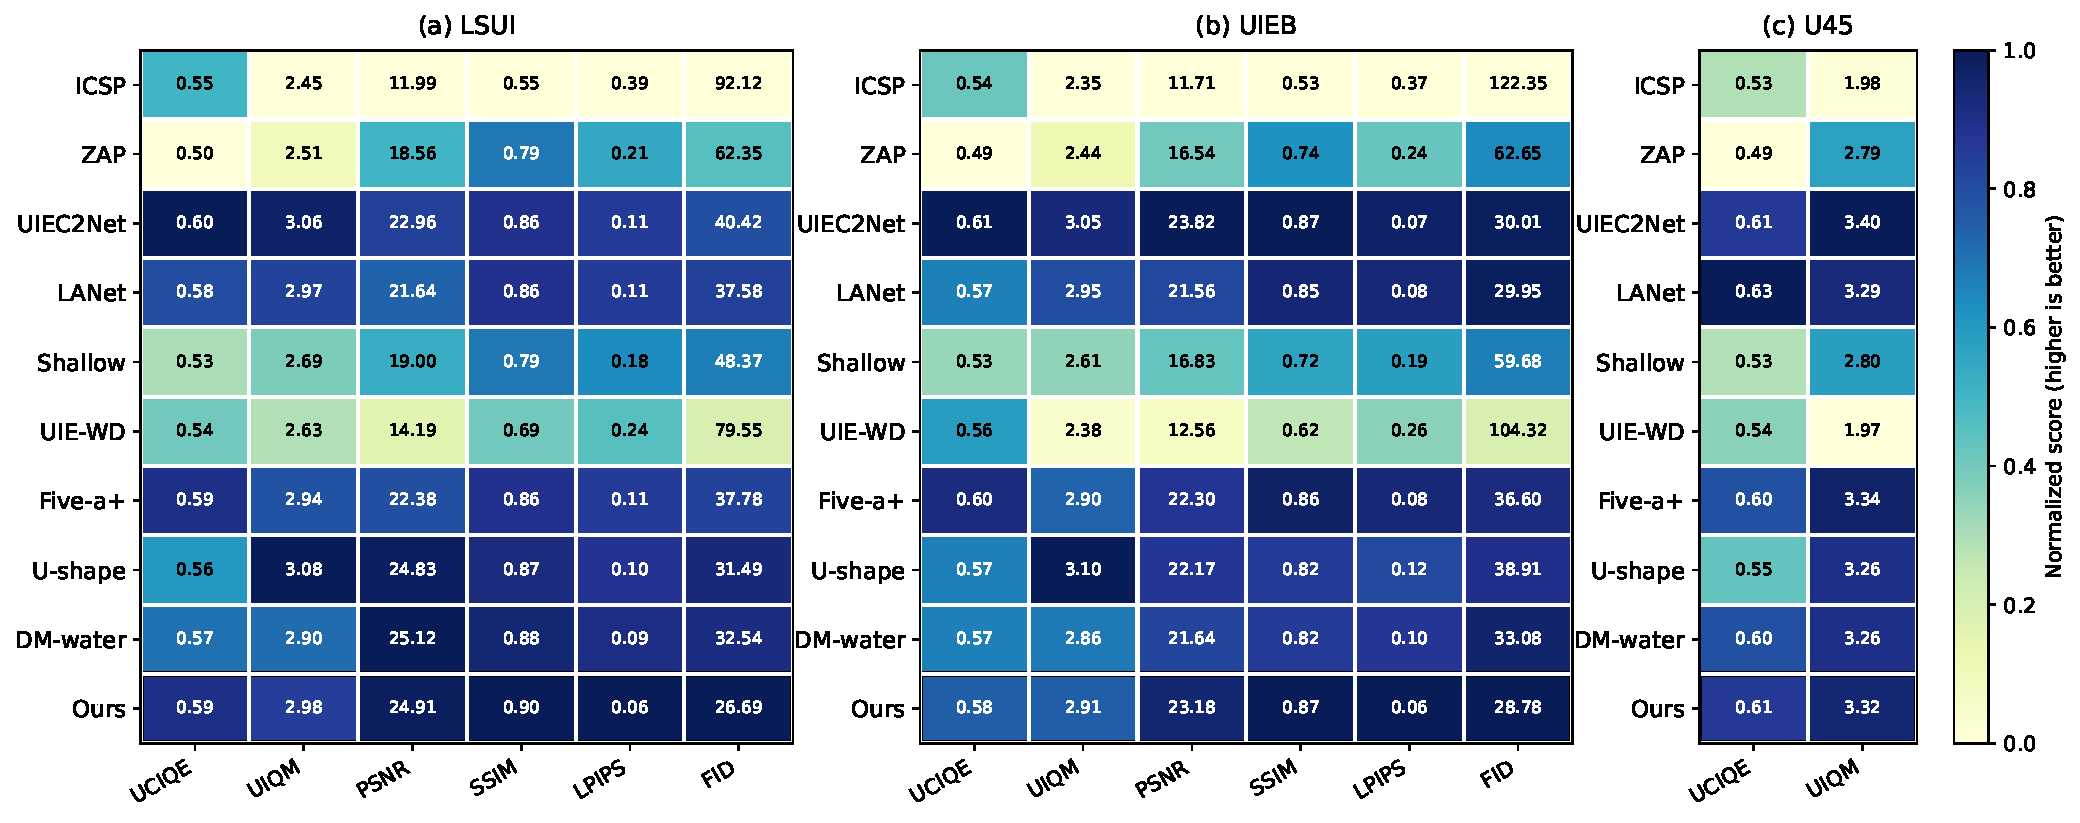
\includegraphics[width=\textwidth]{fig_quant_heatmap.pdf}
    \caption{Large-scale quantitative heatmap across benchmarks and metrics.}
    \label{fig:quant_heatmap_main}
\end{figure*}

\begin{figure*}[htbp]
    \centering
    % trim=左 下 右 上，clip代表开启裁剪。
    \includegraphics[width=\textwidth]{fig4.png}
    \caption{Qualitative comparison of different underwater image enhancement methods. Six typical degraded samples are selected, where the top three rows represent greenish degradations and the bottom three rows represent bluish, heavily scattered degradations.}
    \label{fig:qualitative_comp}
    \vspace{-0.6cm}
\end{figure*}

\subsection{Ablation Study}

We conduct a systematic ablation study on the LSUI dataset to verify our core components and optimal hyperparameters. First, we investigate the impact of inference steps in Table \ref{tab:ablation_steps}. Benefiting from Rectified Flow's constant velocity field estimation, the model achieves decent enhancement with a single forward pass at $N=1$. Increasing the steps to $N=3$ makes the numerical integration more precise, comprehensively improving UCIQE, UIQM, PSNR, and SSIM to a local optimum. However, further increasing steps to $N=10$ degrades pixel-sensitive metrics such as PSNR and SSIM due to accumulated truncation errors and noise. Thus, to balance generation quality and efficiency, we strictly set the testing inference step to 3. A heatmap-style ablation visualization is included in the supplementary material for detailed inspection.



Next, we construct four network variants to evaluate the contributions of physical priors, the two-stage loss, and the Adaptive Masking strategy ADMK, as listed in Table \ref{tab:ablation_modules}. Model I is a pure data-driven baseline using only the Rectified Flow framework. It still surpasses traditional methods, proving the architecture's strong representational capability. Model II explicitly introduces physical priors, namely background light and transmission maps, to guide generation, effectively converging the solution space and elevating UCIQE, UIQM, and PSNR. This confirms their critical role in correcting color casts. Model III integrates the two-stage composite loss, substantially bolstering perceptual capability for local contrast and pushing PSNR and SSIM to peak values of 25.05 and 0.91. Finally, Model IV as our complete algorithm incorporates the ADMK strategy and utilizes binary masks to isolate spatial interference from low-quality training regions. 
% 表4：推理步数消融实验
\begin{table}[t]
    \centering
    \small 
    \caption{Impact of different inference steps on model performance. Red indicates the best value and blue indicates the second best value.}
    \label{tab:ablation_steps}
    \begin{tabular*}{\linewidth}{@{\extracolsep{\fill}}lcccc}
        \toprule
        Inference Steps & UCIQE $\uparrow$ & UIQM $\uparrow$ & PSNR $\uparrow$ & SSIM $\uparrow$ \\
        \midrule
        $N=1$ & 0.56 & 2.90 & 24.13 & \second{0.88} \\
        $N=3$ & \second{0.59} & \second{2.98} & \best{24.91} & \best{0.90} \\
        $N=5$ & \best{0.61} & 2.92 & \second{24.87} & \second{0.88} \\
        $N=10$ & 0.57 & \best{3.01} & 24.65 & 0.86 \\
        \bottomrule
    \end{tabular*}
\end{table}
% 表5：网络模块消融实验
\begin{table}[t]
    \centering
    \small 
    \caption{Ablation study of different modules. Red indicates the best value, blue indicates the second best value, and bold highlights our method only.}
    \label{tab:ablation_modules}
    \begin{tabular*}{\linewidth}{@{\extracolsep{\fill}}lccccccc}
        \toprule
        Model & Conditions & Two-Stage Loss & ADMK & UCIQE $\uparrow$ & UIQM $\uparrow$ & PSNR $\uparrow$ & SSIM $\uparrow$ \\
        \midrule
        Model I   & $\times$   & $\times$       & $\times$ & 0.55 & 2.84 & 24.12 & 0.84 \\
        Model II  & \checkmark & $\times$       & $\times$ & \second{0.58} & \second{2.92} & 24.37 & 0.86 \\
        Model III & \checkmark & \checkmark     & $\times$ & 0.57 & 2.90 & \best{25.05} & \best{0.91} \\
        \midrule
        \textbf{Model IV}  & \textbf{\checkmark} & \textbf{\checkmark} & \textbf{\checkmark} & \textbf{\best{0.59}} & \textbf{\best{2.98}} & \textbf{\second{24.91}} & \textbf{\second{0.90}} \\
        \bottomrule
    \end{tabular*}
\end{table}
Although full-reference metrics PSNR and SSIM experience a marginal drop due to masked pixels, human-aligned no-reference metrics UCIQE and UIQM improve further. More importantly, as demonstrated in Figure \ref{fig:ablation_mask}, ADMK successfully eliminates the abnormal restoration and blurring artifacts common in pure data-driven models, achieving optimal comprehensive visual realism and structural consistency.
\FloatBarrier
% 图5：ADMK 消融视觉对比图
\begin{figure}[H]
    \centering
    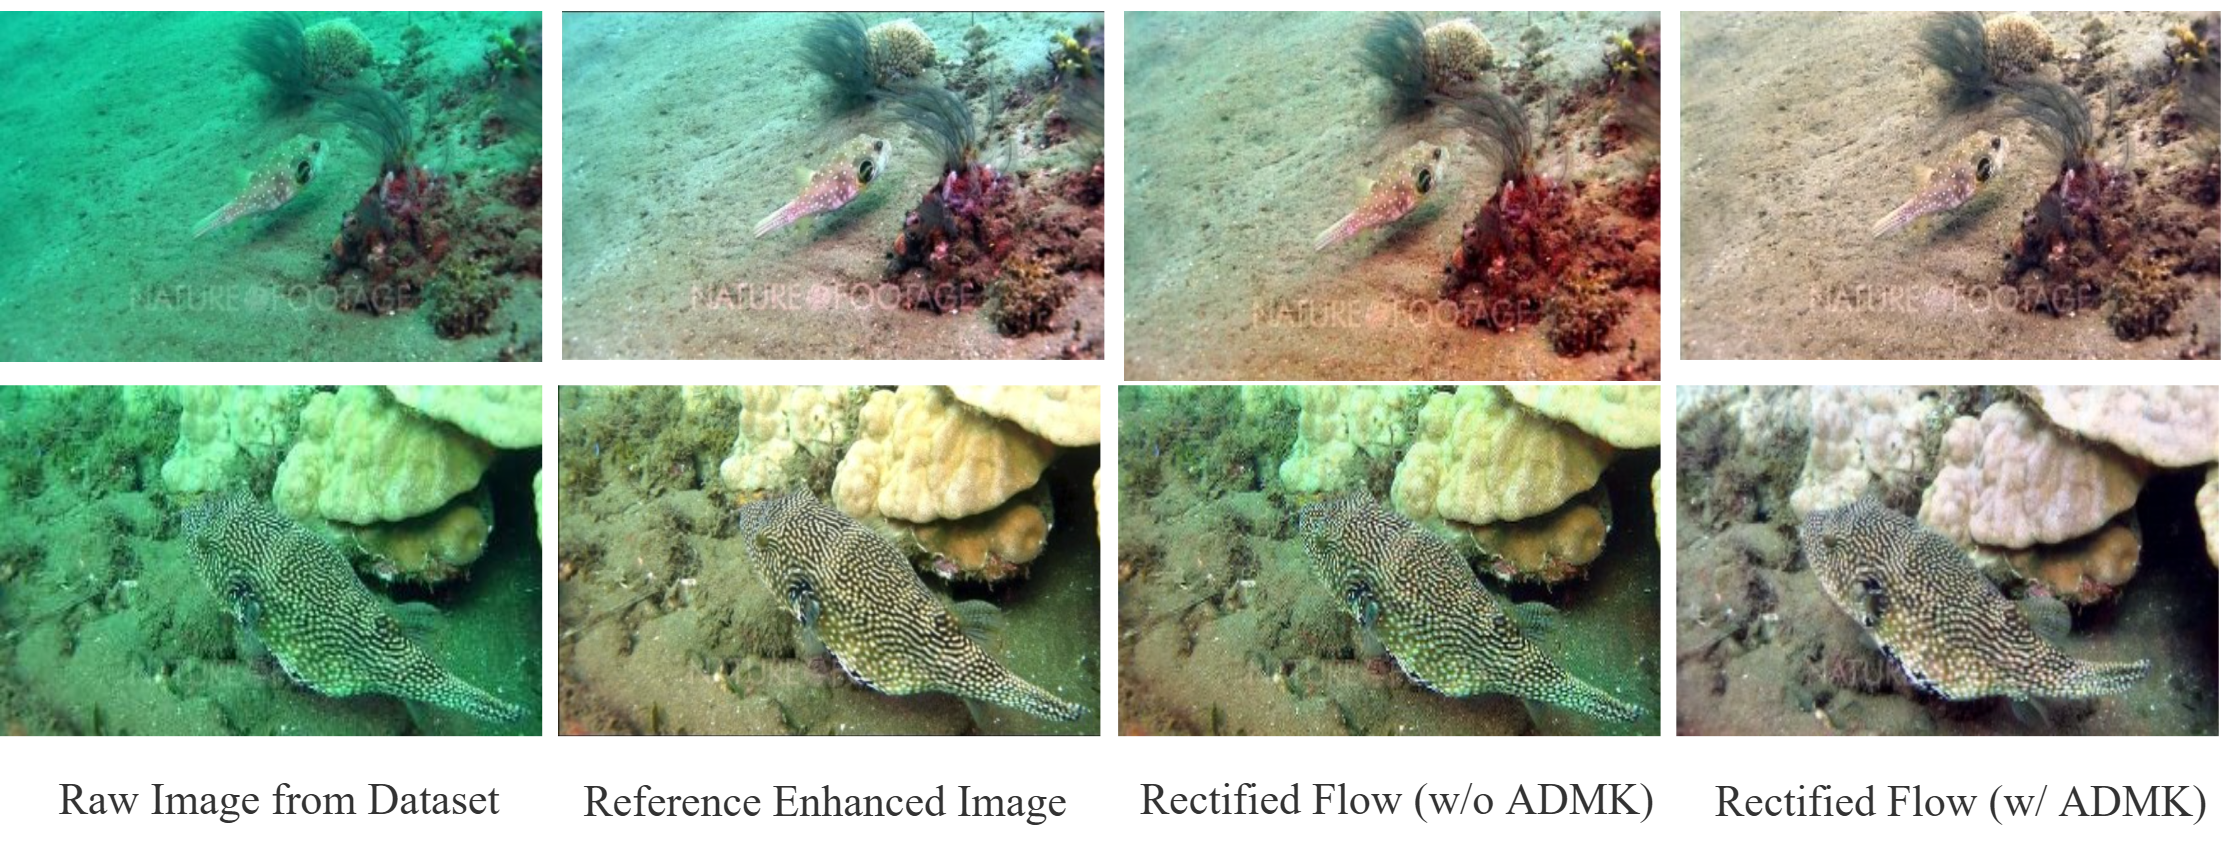
\includegraphics[width=\linewidth]{fig5.png}
    \caption{Visual comparison of underwater image enhancement with and without the Adaptive Masking (ADMK) strategy.}
    \label{fig:ablation_mask}
\end{figure}

% !TeX root = ../main.tex
\subsection{Speed and Efficiency Analysis}
\label{sec:speed}

We further evaluate runtime under the same hardware and input setting used in the main experiments. The comparison includes two representative diffusion baselines, DM-water~\cite{r24} and PA-Diff~\cite{r8}. All settings are evaluated at $512\times512$, and we report latency in milliseconds per image and throughput in frames per second.

\begin{table}[H]
    \centering
    \small
    \caption{Runtime comparison at $512\times512$ resolution. Speedup columns are computed against DM-water and PA-Diff.}
    \label{tab:speed_runtime}
    \setlength{\tabcolsep}{3.5pt}
    \begin{tabular*}{\linewidth}{@{\extracolsep{\fill}}lcccc}
        \toprule
        Setting & Latency (ms) $\downarrow$ & FPS $\uparrow$ & vs DM-water $\uparrow$ & vs PA-Diff $\uparrow$ \\
        \midrule
        Ours ($N=1$) & 99 & 10.10 & 5.66$\times$ & 9.29$\times$ \\
        Ours ($N=3$) & 292 & 3.42 & 1.92$\times$ & 3.15$\times$ \\
        Ours ($N=5$) & 487 & 2.05 & 1.15$\times$ & 1.89$\times$ \\
        DM-water~\cite{r24} & 560 & 1.79 & 1.00$\times$ & 1.64$\times$ \\
        PA-Diff~\cite{r8} & 920 & 1.09 & 0.61$\times$ & 1.00$\times$ \\
        \bottomrule
    \end{tabular*}
\end{table}

Table~\ref{tab:speed_runtime} shows that RF-MCUIE keeps clear efficiency advantages over both diffusion baselines in practical operating points. The three-step setting remains a strong default for quality and runtime. At step $N=5$, the iterative refinement is already complete and the restoration quality is strong, while runtime is still faster than DM-water and PA-Diff.

\FloatBarrier


% !TeX root = ../main.tex
\section{Conclusion}
\label{sec:conclusion}

This research presents a Multi-Condition Underwater Image Enhancement network based on Rectified Flow, referred to as RF-MCUIE, designed to mitigate severe underwater degradations such as color casts and structural blurring. The framework addresses training instabilities through an Adaptive Masking strategy, termed ADMK, which effectively filters low-quality supervision signals. Furthermore, physical priors involving background light and transmission maps are integrated as conditional guidance to ensure the restoration adheres to established optical mechanisms. By leveraging the Rectified Flow regime and a two-stage composite loss, the model establishes a straight-line transport path that facilitates high-fidelity generation within minimal inference steps. Comprehensive experiments on the LSUI, UIEB, and U45 benchmarks demonstrate that the proposed method achieves state-of-the-art performance across various objective metrics, including LPIPS, FID, and UCIQE. Ultimately, RF-MCUIE provides a reliable and efficient solution for bandwidth-limited underwater visual systems by balancing superior restoration quality with significantly reduced computational latency.


% ---- Bibliography ----
%
% BibTeX users should specify bibliography style 'splncs04'.
% References will then be sorted and formatted in the correct style.
%
\bibliographystyle{splncs04}
\bibliography{bibliography/main}
\end{document}
